\documentclass[12pt]{article}
\usepackage{nott-titlepage}

\usepackage{graphicx}
\usepackage{float}
\usepackage[section]{placeins}
\usepackage{aliascnt}
\newaliascnt{eqfloat}{equation}
\newfloat{eqfloat}{h}{eqflts}
\floatname{eqfloat}{Equation}
\usepackage{amsmath}

\newcommand*{\ORGeqfloat}{}
\let\ORGeqfloat\eqfloat
\def\eqfloat{%
  \let\ORIGINALcaption\caption
  \def\caption{%
    \addtocounter{equation}{-1}%
    \ORIGINALcaption
  }%
  \ORGeqfloat
}

\usepackage{siunitx}
\usepackage{listings}

\usepackage{tikz}
\usetikzlibrary {circuits.ee.IEC}
\tikzset{circuit declare symbol=motor}

\usepackage{biblatex}
\bibliography{citation}

\title{Performance of a PMSM Part 2}
\author{Tan Hong Kai}
\date{December 24 2023}
\studentid{20386501}
\module{EEEE3114 Electrical Machines, Drive Systems and Applications}
\department{Department of Electrical and Electronics Engineering}

\begin{document}
\maketitle

\section{Introduction}

A permanent magnet synchronous motor (PMSM) is simulated in FEMM software. The motor is given in a DXF file. However, a modified version of the model is used throughout the simulations conducted using an anti-periodic air gap in FEMM to increase the simulation speeds. A few simulations were conducted in a series of tasks to explore the characteristics of the motor. To further automate the changing of parameters in the model, the FEMM python pyfemm interface were used to collect the data and plot it.

The motor has a rated speed of 1500 rpm with 4 poles (2 pole pairs). It has a rated current of $20$ A peak to peak. The peak torque is at $\ang{90}$ load angle. Each of the poles have 6 slots, each current phase have 2 windings. 

This is the part 2 of the same coursework where the simulations and results of task 7 to task 10 is explored.

\section{Task 7}

The 7th task is to find the equivalent circuit parameters of the synchronous machine. The equivalent circuit is then used to calculate machine performance at rated conditions and compared.

\subsection{Methodology}

The equivalent circuit is made up of 3 different components. The first is the stator winding resistance $R_{s}$. The second is the synchronous inductance $X_{s}$. The last one is the back EMF of the motor $E_{b}$. The equivalent described is shown in figure \ref{fig:eq-circuit-combi}.

\begin{figure}[H]
    \centering
    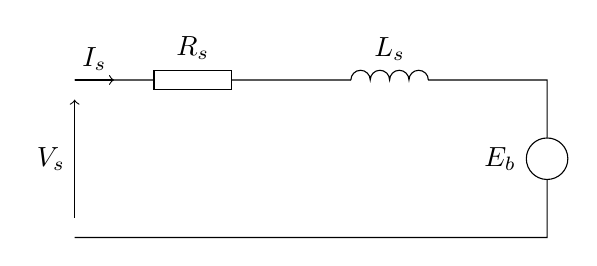
\begin{tikzpicture}[circuit ee IEC,
    set motor graphic={draw, shape=circle, minimum size=15pt}]
        \draw (-1, 0) 
        to [resistor={info=$R_s$}] (2, 0)
        to [inductor={info=$L_s$}] (4, 0)
        to (5, 0)
        to [motor={info=left:$E_b$}] (5, -2)
        to (5, -2) to (-1, -2);

        \draw [->] (-1, -1.75) -- node[anchor=east] {$V_{s}$} (-1, -0.25);
        \draw [->] (-1, 0) -- node[above] {$I_{s}$} (-0.5, 0);
    \end{tikzpicture}
    \caption{Equivalent Circuit of the Synchronous Machine}
    \label{fig:eq-circuit-combi}
\end{figure}

However, the synchronous inductance can be split into two different inductances connected in series. One is the leakage inductance $X_{l}$ and the other is the magnetizing inductance $X_{m}$. The final equivalent circuit is show in figure \ref{fig:eq-circuit}.

\begin{figure}[H]
    \centering
    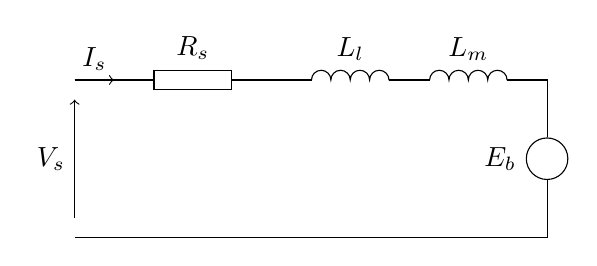
\begin{tikzpicture}[circuit ee IEC,
    set motor graphic={draw, shape=circle, minimum size=15pt}]
        \draw (-1, 0) 
        to [resistor={info=$R_s$}] (2, 0)
        to [inductor={info=$L_l$}] (3, 0)
        to [inductor={info=$L_m$}] (5, 0)
        to [motor={info=left:$E_b$}] (5, -2)
        to (5, -2) to (-1, -2);

        \draw [->] (-1, -1.75) -- node[anchor=east] {$V_{s}$} (-1, -0.25);
        \draw [->] (-1, 0) -- node[above] {$I_{s}$} (-0.5, 0);
    \end{tikzpicture}
    \caption{Complete Equivalent Circuit of the Synchronous Machine}
    \label{fig:eq-circuit}
\end{figure}

The stator winding resistance $R_{s}$ can be obtained in FEMM by obtaining the voltage drop in the circuit properties and dividing the real part of the voltage by the current. 

\begin{equation}
    R_s = \frac{V_{drop}}{I_{s}}
\end{equation}

The synchronous inductance can be obtained in FEMM by getting the flux linkage in the circuit and dividing it by the current of the circuit. This has to be done when the load angle is at 90 and at a rotor angle with the maximum flux linkage.

The leakage inductance can be obtained similar to synchronous inductance. However, the flux linkage value is obtained with the permanent magnet with air instead of N42. With the leakage inductance, the magnetizing inductance can be obtained by subtracting synchronous inductance with leakage inductance.

\begin{equation}
    L = \frac{\lambda}{I_{s}}
\end{equation}

\FloatBarrier

\subsection{Results}

\begin{figure}[H]
    \centering
    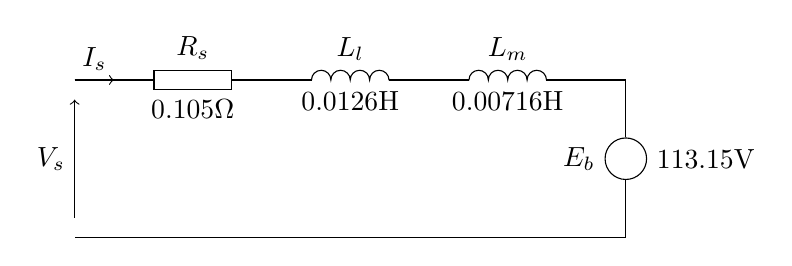
\begin{tikzpicture}[circuit ee IEC,
    set motor graphic={draw, shape=circle, minimum size=15pt}]
        \draw (-1, 0) 
        to [resistor={info=$R_s$, ohm'=0.105}] (2, 0)
        to [inductor={info=$L_l$, henry'=0.0126}] (3, 0)
        to [inductor={info=$L_m$, henry'=0.00716}] (6, 0)
        to [motor={info=left:$E_b$, info'=right:{113.15V}}] (6, -2)
        to (6, -2) to (-1, -2);

        \draw [->] (-1, -1.75) -- node[anchor=east] {$V_{s}$} (-1, -0.25);
        \draw [->] (-1, 0) -- node[above] {$I_{s}$} (-0.5, 0);
    \end{tikzpicture}
    \caption{Equivalent Circuit of the Synchronous Machine}
    \label{fig:eq-circuit-results}
\end{figure}

\FloatBarrier

\subsection{Checking Results \& Comparison}

The theoretical results can be calculated to double-check the obtained values. The theoretical reactance can be calculated using the power developed equation (equation \ref{eq:power-dev}). Substituting $V_{s}$ equation in equation \ref{eq:voltage-value} derived from phasor diagram \ref{fig:vs-phasor}. The phasor diagram shows the $V_{s}$ at \ang{90} load angle and assumes the armature resistance is negligible.

\begin{equation} \label{eq:power-dev}
    P_{d} = 3 \frac{E V_{s}}{X_{s}} \sin{\delta}
\end{equation}

\begin{equation} \label{eq:voltage-value}
    V_{s} = \sqrt{(I_{s} X_{s})^{2} - E_{b}^{2}}
\end{equation}

\begin{figure}[H]
    \centering
    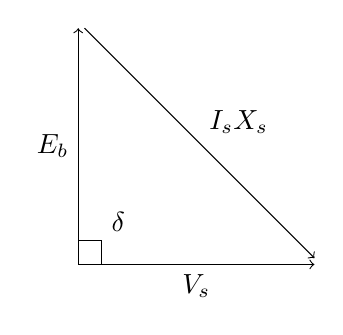
\begin{tikzpicture} \label{fig:vs-phasor}
        \draw [->] (0, 0) -- node[left] {$E_{b}$} (0, 3);
        \draw [->] (0, 0) -- node[below] {$V_{s}$} (3, 0);
        \draw [->] (0.08, 3) -- node[above right] {$I_{s} X_{s}$} (3, 0.08);
        \draw (0, 0.3) -- (0.3, 0.3) node[above right] {$\delta$} -- (0.3, 0);
    \end{tikzpicture}
    \caption{Phasor Diagram of the Machine}
\end{figure}

Solving for $X_{s}$:

\begin{center}
    \begin{align*}
        X_{s} &= \sqrt{\frac{I_{s}^{2} - \frac{P^{2}}{9 E_{b}^{2}}}{E^{2}}}^{-1}\\
            &= \sqrt{\frac{20^{2} - \frac{2340.487}{9 * 113.2^{2}}}{113.2^{2}}}^{-1}\\
            &= 6.029 \Omega
    \end{align*}
\end{center}

The measured $X_{s}$ for the equivalent circuit would be:

\begin{center}
    \begin{align*}
        X_{s} &= 2\pi{}f(L_{l} + L_{m})\\
            &= 2 * \pi * 50 * (0.0126 + 0.00716)\\
            &= 6.208 \Omega
    \end{align*}
\end{center}

The measured value is higher due to additional losses considered using FEMM.

\subsubsection{Power}

Using both the calculated value, the power can be calculated.

FEMM (at \ang{90} load angle):

\begin{center}
    \begin{align*}
        P_{d} &= T \omega\\
           &= 14.9 * 1500 * 2 * \pi / 60\\
            &= 2340.487 W
    \end{align*}
\end{center}

Equivalent Circuit:

\begin{center}
    \begin{align*}
        P_{d} &= 3 * \frac{113.2 * \sqrt{(20 * 6.208)^{2} - 113.2^{2}}}{6.208} \sin{\ang{90}}\\
            &= 2790.134 W
    \end{align*}
\end{center}

Comparison:

\begin{center}
    \begin{equation*}
        \frac{2790.134 - 2340.487}{270.134} * 100\% = 16.115\%
    \end{equation*}
\end{center}

The equivalent circuit has 16.115\% (\~450 W) more power due to the losses in FEMM. 

\subsubsection{Power Factor}

\begin{center}
    \begin{align*}
        P_{d} &= 3 V_{s} I_{s} \cos{\phi}\\
        \cos{\phi} &= \frac{P_{d}}{3 V_{s} I_{s}}\\
            &= \frac{2790.134}{3 * 20 \sqrt{(20 * 6.208)^{2} - 113.2^{2}}}\\
            &= 0.911
    \end{align*}
\end{center}

\section{Task 8}

The 8th task is to explore motor output torque as a function of the load angle. Both output torque from simulation in FEMM and equivalent circuit are explored. The differences between the two graph are compared.

\subsection{Methodology}

The simulated values can be obtained by changing the current in the circuit with different load angle. The torque is then extracted at that current. To ensure the rated torque aligns, the rotor is rotated so that the torque developed would be 0 at a load angle of \ang{0}.

The output torque from the equivalent circuit can be obtained by using equation \ref{eq:circuit-td}. This is derived from the power developed equations \ref{eq:pd-1} and \ref{eq:pd-2}. The load angle is then varied, and the torque values are recorded. \textbf{Note} that these equations assume the synchronous motor operates in the linear region of the B-H curve in the stator core.

\begin{eqfloat}
    \begin{equation}\label{eq:circuit-td}
        T = 3 \frac{E_{b}V_{s}}{X_{s}\omega{}} \sin{\delta} 
    \end{equation}
    \begin{equation}\label{eq:pd-1}
        P_{d} = 3 \frac{E_{b}V_{s}}{X_{s}} \sin{\delta} 
    \end{equation}
    \begin{equation}\label{eq:pd-2}
        P_{d} = T \omega
    \end{equation}
    \caption{Equations Used for Torque Developed}
\end{eqfloat}

\subsection{Results}

\begin{figure}[H]
    \centering
    \includegraphics[width=\linewidth]{img/task_8_simulation.png}
    \caption{Torque Output Using FEMM}
    \label{fig:task-8-simulation}
\end{figure}

\begin{figure}[H]
    \centering
    \includegraphics[width=\linewidth]{img/task_8_circuit.png}
    \caption{Torque Output Using Equivalent Circuit}
    \label{fig:task-8-circuit}
\end{figure}

\subsection{Analysis}

The peak torque is negative at a load angle of \ang{90} in the FEMM. This is due to the direction of magnetic field and rotor angle during simulation in FEMM. However, the shape of the torque output remains the for both FEMM and equivalent circuit. This can be ignored as the only difference would be in signage.

Even though the theoretical peak torque should be at $\ang{90}$ load angle, the simulated torque output using FEMM is slightly different at $\ang{77}$. This is due to the non-linear B-H curve of the stator and rotor materials. 

The peak torque is different from the values obtained from the equivalent circuit, where the peak torque is exactly at \ang{90} load angle. The equivalent circuit values didn't take into considerations the B-H curve of the magnetic materials. Assuming, operation in the linear region of the B-H curve results in higher peak torque, as there are fewer losses in the model.

\section{Task 9}

The 9th task is to explore the effects of the magnet pitch factor on the motor performance (back EMF and rated torque) and air gap flux density. The pitch factor is how much of the pole is covered by the magnet.

The pitch factor of 0.01, 0.1, 0.2, 0.3, 0.4, 0.45, 0.5, 0.6, 0.7, 0.8, 0.9, 1.0 are explored.

\subsection{Methodology}

The magnet pitch factor can be varied by moving the points of the magnet to make it cover the area needed. The simulations are then carried out with the new pitch factors. 

The air gap flux density can be obtained using the \lstinline{mo_getgapb} function. The method of obtaining performance metrics were described in the previous report.

\begin{figure}[H]
    \centering
    \includegraphics[height=0.8\linewidth, trim={0 0 30cm 1}, clip]{img/task_9_models/task_9_0.01.png}
    \caption{Model at Pitch Factor of 0.01}
    \label{fig:task-9-0.01-pf}
\end{figure}

\begin{figure}[H]
    \centering
    \includegraphics[height=0.8\linewidth, trim={0 0 31cm 1.5}, clip]{img/task_9_models/task_9_1.0.png}
    \caption{Model at Pitch Factor of 1}
    \label{fig:task-9-1-pf}
\end{figure}

\subsection{Results}

\begin{figure}[H]
    \centering
    \includegraphics[width=\linewidth]{img/task_9_airgap_flux.png}
    \caption{Air Gap Flux Density at Different Pitch Factor}
    \label{fig:task-9-airgap-flux}
\end{figure}

\begin{figure}[H]
    \centering
    \includegraphics[width=\linewidth]{img/task_9_back_emf.png}
    \caption{Back EMF at Different Pitch Factor}
    \label{fig:task-9-back-emf}
\end{figure}

\begin{figure}[H]
    \centering
    \includegraphics[width=\linewidth]{img/task_9_torque.png}
    \caption{Rated Torque at Different Pitch Factor}
    \label{fig:task-9-torque}
\end{figure}

\subsection{Analysis}

The air gap flux density increases linearly as the pitch factor increases. This is due to the increase in area of the magnet. More of the air gap is covered by the magnet, hence increasing the flux density.

The back EMF increases linearly until the pitch factor of 0.3 is reached. The back EMF remains relatively constant no matter the pitch factor. This is due to the flux density in the stator teeth increasing. However, the core saturates after the pitch factor reaches 0.3. The back EMF is proportional to the flux density (Faraday's Law of Induction).

\begin{eqfloat}[H]
    \begin{equation}\label{eq:faradays}
        EMF = - N \frac{d\phi}{dt}
    \end{equation}
    \caption{Faraday's Law of Induction}
\end{eqfloat}

The rated torque increases in a linear form as the pitch factor increases. This is due to the increase in air gap flux density. However, the plot is not entirely linear as due to the non-linearity of B-H curve of the stator core.

\section{Task 10}

The 10th task is to vary the opening slot factor (the variation between slot width and slot opening width) of the synchronous machine. The torque developed (ripple and mean) and the cogging torque are compared.

The slot factor of 0.1, 0.2, 0.3, 0.4, 0.5, 0.6, 0.7, 0.8, 0.9, 1.0 are explored.

\subsection{Methodology}

The opening slot factor can be varied by moving the slot edge nodes closer or further apart. This can be done by rotating the nodes by the angle needed for the new opening slot factor.

The torque ripple is measured the same as task 3 by varying the load angle and rotating the rotor by \ang{0.5} for every \ang{1} changing in load angle. The cogging torque can be measured when the circuit is at 0 A (same as task 1).

\begin{figure}[H]
    \centering
    \includegraphics[height=0.8\linewidth, trim={0 0 22.5cm 1}, clip]{img/task_10_models/task_10_0.1.png}
    \caption{Model at Slot Factor of 0.1}
    \label{fig:task-10-0.1-sf}
\end{figure}

\begin{figure}[H]
    \centering
    \includegraphics[height=0.8\linewidth, trim={0 0 29cm 185}, clip]{img/task_10_models/task_10_1.0.png}
    \caption{Model at Slot Factor of 1}
    \label{fig:task-9-1-sf}
\end{figure}


\subsection{Results}

\begin{figure}[H]
    \centering
    \includegraphics[width=\linewidth]{img/task_10_overall_torque.png}
    \caption{Mean Torque at Different Opening Slot Factor}
    \label{fig:task-10-torque}
\end{figure}

\begin{figure}[H]
    \centering
    \includegraphics[width=\linewidth]{img/task_10_ripple_amplitude.png}
    \caption{Torque Ripple Amplitude at Different Opening Slot Factor}
    \label{fig:task-10-ripple-amp}
\end{figure}

\begin{figure}[H]
    \centering
    \includegraphics[width=\linewidth]{img/task_10_torque_ripple.png}
    \caption{Torque Ripple Waveform at Various Opening Slot Factor}
    \label{fig:task-10-ripple}
\end{figure}

\begin{figure}[H]
    \centering
    \includegraphics[width=\linewidth]{img/task_10_cogging_amplitude.png}
    \caption{Cogging Torque Amplitude at Different Opening Slot Factor}
    \label{fig:task-10-cogging-amp}
\end{figure}

\begin{figure}[H]
    \centering
    \includegraphics[width=\linewidth]{img/task_10_cogging_torque.png}
    \caption{Cogging Torque Waveform at Various Opening Slot Factor}
    \label{fig:task-10-cogging}
\end{figure}

\subsection{Analysis}

The mean torque developed by the machine increase with a higher slot factor, up to a slot factor of around 0.3. This is due to the increase in the effectiveness of the magnetic coupling. However, as the slot factor increases, less magnetic coupling happening causing the torque developed decreases.

The torque ripple and cogging torque amplitude is higher at higher slot opening factor. This is due to the leakage flux density and the non-homogeneousness of the air gap flux density when the tooth shoe/tip becomes smaller. The leakage flux causes unwanted torque to developed on the rotor. This is called the slotting effect. However, when the slot factor is low, the ineffective magnetic coupling also causes the same issues. \cite{task-10}

\clearpage

\printbibliography

\end{document}
